%main.tex
\documentclass[a4paper,11pt,twoside,ngerman,color]{book}
% header.tex

% Korrekte Darstellung der Umlaute (language and fonts)
\usepackage[T1]{fontenc} % T1-Fonts are better
\usepackage{lmodern} % Eine etwas angenehmere Font
\usepackage[utf8]{inputenc} % nutzt UTF8, bitte was sonst
\usepackage[main=ngerman]{babel} % Übersetze einige Literate auf Deutsch

% Math and theoretical computer science symboles/fonts
\usepackage{amsmath}  % American Math Society Packete: general
\usepackage{amsfonts} % American Math Society Packete: more fonts
\usepackage{amssymb}  % American Math Society Packete: more symbols
%\usepackage{amsthm}  % American Math Society Packete: typesetting theorems  %%% in conflict with ntheorem!!!
\usepackage{stmaryrd} % St Mary Road symbols for theoretical computer science
\usepackage{dsfont}   % supports the 1-function

% Caption Packet
\usepackage[margin=0pt,font=small,labelfont=bf]{caption} % cus­tomise the cap­tions in float­ing en­vi­ron­ments
% Gliederung einstellen
%\setcounter{secnumdepth}{5}
%\setcounter{tocdepth}{5}

% citations/ captions/ float­ing en­vi­ron­ments/ links
\usepackage{cite} % Improved Citation-Handling
\usepackage[babel,german=quotes,autostyle]{csquotes} % ad­vanced fa­cil­i­ties for in­line and dis­play quo­ta­tions
\MakeOuterQuote{"}	% for german style quotation marks
\usepackage{subcaption} % Support for sub-captions (and sub-figures)
\usepackage{enumerate} % Erweiterte Enumerate-Umgebungen
\usepackage{wrapfig} % Erlaubt es Text, Graphiken zu umfließen
\usepackage{lscape}
\usepackage{rotating}
%\usepackage{epstopdf}
\usepackage{float} % Verbesserte floating-objects
\usepackage{framed} % Umrahmte Abschnitte
\usepackage[framed,hyperref,amsmath,thmmarks]{ntheorem} % en­hance­ments for the­o­rem-like en­vi­ron­ments
\usepackage[unicode,pdfmenubar,linktoc=all,hidelinks,bookmarks]{hyperref} % ermöglicht PDF-Verklinkungen
\usepackage{url} % al­lows line­breaks at cer­tain char­ac­ters in urls/ e-mail adresses/ paths
\usepackage{multicol} % to use columns with multiple rows

% Abkuerzungen richtig formatieren %
\usepackage{xspace}

% Euro Symbol
\usepackage{eurosym}

% Seitenlayout
\usepackage{geometry} % Beinflusst das Seitenlayout
\geometry{a4paper} % Papiergroesse
%%\geometry{top=25mm, inner=25mm, outer=25mm, bottom=25mm, headsep=10mm, footskip=10mm} % Seitenraender
%%\geometry{left=3.5cm,right=2.5cm,bottom=3.5cm,top=3cm} % Seitenraender
\usepackage{pdflscape} % Landscape Umgebung für PDF Dokumente: set­ting the page at­tribute /Ro­tate 
\usepackage[hang]{footmisc}   % Für den Einzug bei Fußnoten
\setlength{\footnotemargin}{0pt} % Setze den Einzug für die Fußnoten
\parskip 0pt
%\parindent 0pt

% Grafiken
\usepackage[pdftex]{color} % Erweiterter Support für Graphiken
\usepackage{graphicx}
%\usepackage{subfigure}
\usepackage{tikz} % Für LaTeX Graphiken
\usetikzlibrary{automata,arrows,backgrounds,decorations.markings,decorations.pathmorphing,decorations.pathreplacing,fit,positioning,shadows,shapes,shapes.geometric} % Ein paar nützliche TikZ-Pakete


% Bibtex deutsch
\usepackage{bibgerm}

\usepackage{makeidx} % Index für Schlagwörter
\makeindex

\usepackage[final]{listofsymbols}  % Symbolverzeichnis
%\usepackage[draft]{listofsymbols}


% Zeilenabstand einstellen %
\renewcommand{\baselinestretch}{1.25}
% Floating-Umgebungen anpassen %
\renewcommand{\topfraction}{0.9}
\renewcommand{\bottomfraction}{0.8}

% Keine einzelnen Zeilen beim Anfang eines Abschnitts (Schusterjungen)
\clubpenalty = 10000
% Keine einzelnen Zeilen am Ende eines Abschnitts (Hurenkinder)
\widowpenalty = 10000 \displaywidowpenalty = 10000
% EOF

 % Seitenraender %
\geometry{left=3.5cm,right=2.5cm,bottom=3.5cm,top=3cm}

% Algorithmen
\usepackage[plain,chapter]{algorithm}
\usepackage{algorithmic}
%\usepackage{algpseudocode}

% Tabellen
%\usepackage{booktabs}  % Statt \hline kann \toprule, \midrule und \bottomrule verwendet werden.
%\usepackage{multirow} % provides a construction for table cells that span more than one row
%\usepackage{multicol} % allows switching between one and multicolumn format on the same page

% theoremOptions.tex

% Theorem-Optionen %
\theoremseparator{.}
\theoremstyle{change}
\newtheorem{theorem}{Theorem}[section]
\newtheorem{satz}[theorem]{Satz}
\newtheorem{lemma}[theorem]{Lemma}
\newtheorem{korollar}[theorem]{Korollar}
\newtheorem{proposition}[theorem]{Proposition}
% Ohne Numerierung
\theoremstyle{nonumberplain}
\renewtheorem{theorem*}{Theorem}
\renewtheorem{satz*}{Satz}
\renewtheorem{lemma*}{Lemma}
\renewtheorem{korollar*}{Korollar}
\renewtheorem{proposition*}{Proposition}
% Definitionen mit \upshape
\theorembodyfont{\upshape}
\theoremstyle{change}
\newtheorem{definition}[theorem]{Definition}
\theoremstyle{nonumberplain}
\renewtheorem{definition*}{Definition}
% Kursive Schrift
\theoremheaderfont{\itshape}
\newtheorem{notation}{Notation}
\newtheorem{konvention}{Konvention}
\newtheorem{bezeichnung}{Bezeichnung}
\theoremsymbol{\ensuremath{\Box}}
\newtheorem{beweis}{Beweis}
\theoremsymbol{}
\theoremstyle{change}
\theoremheaderfont{\bfseries}
\newtheorem{bemerkung}[theorem]{Bemerkung}
\newtheorem{beobachtung}[theorem]{Beobachtung}
\newtheorem{beispiel}[theorem]{Beispiel}
\newtheorem{problem}{Problem}
\theoremstyle{nonumberplain}
\renewtheorem{bemerkung*}{Bemerkung}
\renewtheorem{beispiel*}{Beispiel}
\renewtheorem{problem*}{Problem}
%EOF
% algorithmOptions.tex

% Algorithmen anpassen %
\renewcommand{\algorithmicrequire}{\textbf{Eingabe:}\@\xspace}
\renewcommand{\algorithmicensure}{\textbf{Ausgabe:}\@\xspace}
\floatname{algorithm}{Algorithmus}
\renewcommand{\listalgorithmname}{Algorithmenverzeichnis}
\renewcommand{\algorithmiccomment}[1]{\hfill\color{gray}{// #1}\color{black}}
%EOF
%% pseudoCodeOptions.tex

% pseudocode Einstellungen
\usepackage{listings} % for type­set pro­gram­ming code
\lstset{
  language=Java,
  basicstyle=\ttfamily,
  commentstyle=\color{darkgreen},
  keywordstyle=\bfseries\color{darkblue},
  stringstyle=\color{darkred},
  showspaces=false,
  showstringspaces=false,
  showtabs=false,
  columns=fixed,
  frame=single,
  numbers=left,
  numberstyle=\tiny,
  numbersep=5pt,
  breaklines=true,
  backgroundcolor=\color{lightblue},
  captionpos=b
}
% Python style for highlighting
\newcommand\pythonstyle{\lstset{
language=Python,
basicstyle=\ttm,
otherkeywords={self},             % Add keywords here
keywordstyle=\ttb\color{deepblue},
emph={MyClass,__init__},          % Custom highlighting
emphstyle=\ttb\color{deepred},    % Custom highlighting style
stringstyle=\color{deepgreen},
frame=tb,                         % Any extra options here
showstringspaces=false            % 
}}
%EOF
% customCommands.tex
\usepackage{xparse}


% shortcuts for mathstuff
\newcommand{\Bed}{\mid}
\newcommand{\Oder}{\ \vee \ }
\newcommand{\Und}{\ \wedge \ }
\newcommand{\argmax}{\text{argmax}}
\newcommand{\GDW}{\Leftrightarrow}
\newcommand{\gdw}{genau dann, wenn\@\xspace}

% Abkuerzungen richtig formatieren %
\newcommand{\vgl}{vgl.\@\xspace} 
\newcommand{\zB}{z.\nolinebreak[4]\hspace{0.125em}\nolinebreak[4]B.\@\xspace}
\newcommand{\bzw}{bzw.\@\xspace}
\newcommand{\dahe}{d.\nolinebreak[4]\hspace{0.125em}h.\nolinebreak[4]\@\xspace}
\newcommand{\etc}{etc.\@\xspace}
\newcommand{\evtl}{evtl.\@\xspace}
\newcommand{\insb}{insb.\@\xspace}
\newcommand{\ggf}{ggf.\@\xspace}
\newcommand{\bzgl}{bzgl.\@\xspace}
\newcommand{\so}{s.\nolinebreak[4]\hspace{0.125em}\nolinebreak[4]o.\@\xspace}
\newcommand{\iA}{i.\nolinebreak[4]\hspace{0.125em}\nolinebreak[4]A.\@\xspace}
\newcommand{\sa}{s.\nolinebreak[4]\hspace{0.125em}\nolinebreak[4]a.\@\xspace}
\newcommand{\sAbb}{s.\nolinebreak[4]\hspace{0.125em}\nolinebreak[4]Abb.\@\xspace}
\newcommand{\sS}{s.\nolinebreak[4]\hspace{0.125em}\nolinebreak[4]S.\@\xspace}
\newcommand{\su}{s.\nolinebreak[4]\hspace{0.125em}\nolinebreak[4]u.\@\xspace}
\newcommand{\ua}{u.\nolinebreak[4]\hspace{0.125em}\nolinebreak[4]a.\@\xspace}
\newcommand{\og}{o.\nolinebreak[4]\hspace{0.125em}\nolinebreak[4]g.\@\xspace}
\newcommand{\oBdA}{o.\nolinebreak[4]\hspace{0.125em}\nolinebreak[4]B.\nolinebreak[4]\hspace{0.125em}d.\nolinebreak[4]\hspace{0.125em}A.\@\xspace}
\newcommand{\OBdA}{O.\nolinebreak[4]\hspace{0.125em}\nolinebreak[4]B.\nolinebreak[4]\hspace{0.125em}d.\nolinebreak[4]\hspace{0.125em}A.\@\xspace}
\newcommand{\engl}{engl.\@\xspace}
\newcommand{\Abb}{Abb.\@\xspace}

% Leere Seite ohne Seitennummer, naechste Seite rechts
\newcommand{\blankpage}{
 \clearpage{\pagestyle{empty}\cleardoublepage}
}
%EOF
%symbols.tex
\opensymdef
\newsym[Menge aller nat"urlichen Zahlen ohne die Null]{symnz}{\mathds{N}}
\newsym[Menge aller nat"urlichen Zahlen einschlie"slich Null]{symnzmn}{\mathds{N}_{0}}
\newsym[Menge aller ganzen Zahlen]{GZ}{\mathds{Z}}
\newsym[Menge aller rationalen Zahlen]{RatZ}{\mathds{Q}}
\newsym[Menge aller reellen Zahlen]{RZ}{\mathds{R}}
\newsym[euklidische Ebene]{RE}{\mathds{R}^2}
\newsym[Graph]{Graph}{G}

\closesymdef


% % % % % % % % % % % % % % % % % % % % % % % % % % % % % % % % % % % % % % % % % % % % % % %
% HIER eigene Angaben ERGÄNZEN:
% % % % % % % % % % % % % % % % % % % % % % % % % % % % % % % % % % % % % % % % % % % % % % %
% title.tex

\newcommand{\MeinVorame}{Julian\@\xspace}
\newcommand{\MeinNachname}{Sauer\@\xspace}
\newcommand{\MeineMatrikelnummer}{197859\@\xspace}

\newcommand{\MeineArbeit}{Masterarbeit\@\xspace}
%\newcommand{\MeineArbeit}{Masterarbeit\@\xspace}

\newcommand{\MeinTitel}{Effiziente Berechnung von $K_5$-Minoren in Graphen}

%\newcommand{\Erstbetreuer}{Name des Erstbetreuers}
\newcommand{\Erstbetreuer}{Prof.\ Dr.\ Petra Mutzel}
%\newcommand{\Erstbetreuer}{Prof.\ Dr.\ Sven Rahmann}
%\newcommand{\Erstbetreuer}{Prof.\ Dr.\ Günter Rudolph}
%\newcommand{\Erstbetreuer}{Prof.\ Dr.\ Johannes Fischer}
\newcommand{\Zweitbetreuer}{Prof.\ Dr.\ Jens Schmidt}
%EOF

% % % % % % % % % % % % % % % % % % % % % % % % % % % % % % % % % % % % % % % % % % % % % % %

\begin{document}
% Titelseite
\begin{titlepage}
\vspace*{-2cm}
\newlength{\links}
\setlength{\links}{-1.5cm}
\sf
\LARGE

\hspace*{\links}
\begin{minipage}{12.5cm}

\includegraphics[width=8cm]{bilder/tulogo-rgb}
%\hspace*{-0.25cm} \textbf{TECHNISCHE UNIVERSITÄT DORTMUND}\\
%\hspace*{-1.2cm} \rule{5mm}{5mm} \hspace*{0.1cm} FACHBEREICH INFORMATIK\\
\end{minipage}

\vspace*{4cm}

\hspace*{\links}
\hspace*{-0.2cm}
\begin{minipage}{8.5cm}
\large
\begin{center}
{\Large \MeineArbeit} \\
\vspace*{1cm}
\bf{ \MeinTitel } \\
\vspace*{1.5cm}
\MeinVorame \MeinNachname\\
\today
\end{center}
\end{minipage}

\vspace*{3.7cm}

\hspace*{\links}

\vspace*{1.5cm}

\vspace*{.6cm}

\hspace*{\links}
\begin{minipage}[b]{5cm}
\normalsize
\raggedright
Betreuer: \\
\Erstbetreuer \\
\Zweitbetreuer \\
\end{minipage}

\definecolor{TUGreen}{rgb}{0.517,0.721,0.094}
\vspace*{2.5cm}
\hspace*{\links}
\begin{minipage}[b]{8cm}
\normalsize
\raggedright
Fakultät für Informatik\\
Algorithm Engineering (LS 11)\\
Technische Universität Dortmund \\
http://ls11-www.cs.tu-dortmund.de
\end{minipage}


\end{titlepage}

\blankpage
%\include{chapters/titelseite_innen}
%\blankpage

\pagenumbering{roman}
\tableofcontents
\cleardoublepage
\pagenumbering{arabic}

% Kapitel
% einleitung.tex
\chapter{Einleitung}
\label{cha:einleitung}

Im Rahmen dieser Masterarbeit wird ein Algorithmus erklärt und implementiert, der entscheiden kann, ob ein Graph \kf-Minor-frei ist.
Er basiert auf einem von Kezdy und McGuinness \cite{KeM92} vorgestellten Algorithmus, der quadratische Laufzeitkomplexität besitzt.

\section{Motivation und Hintergrund}
\label{sec:motivation_und_hintergrund}
Durch die Berechnung von \kf-Minoren kann entschieden werden, ob ein Graph \kf-Minor-frei ist.
Das ist insofern interessant, als dass einige Algorithmen effizienter auf \kf-Minor-freien Graphen ausgeführt werden können.
So ist die Berechnung eines \emph{maximalen Schnittes} (\emph{Max-Cut Problem}) - also das Aufteilen der Knoten eines Graphen in zwei Mengen, sodass die Kanten zwischen diesen beiden Mengen in Summe ein maximales Gewicht besitzen - NP-schwer\cite{Kar72}.
Allerdings wird etwa in \cite{Bar83} gezeigt, dass es für Graphen ohne \kf-Minor in Polynomialzeit gelöst werden kann.
Viele kombinatorische Optimierungsprobleme wie quadratische 0-1 Probleme können als Max-Cut Probleme formuliert werden\cite{BJR89}, sodass \kf-Minor-freie Probleminstanzen deutlich effizienter gelöst werden können.

In \cite{JLMR+19} transformieren Jünger et al.\nolinebreak[4]\@\xspace Ising Spin Glass Probleme zu Max-Cut Problemen, um mit Hilfe von einem Branch-and-Cut Algorithmus eine optimale Lösung zu finden.
Diese kann mit den heuristischen Lösungen, die etwa auf dem Quantencomputer \emph{D-Wave 2000Q} berechnet werden, verglichen werden.
Dadurch kann beispielsweise bewertet werden, ob für die schnellere Laufzeit des Quantencomputers die heuristische Lösung tragbar ist.
Innerhalb des exakten Verfahrens stellen die \kf-Minoren die Schwierigkeit des Problems dar.
Deshalb kann das Problem einerseits für \kf-Minor-freie Graphen effizient gelöst werden.
Andererseits können einer oder mehrere gefundene \kf-Minoren benutzt werden, um innerhalb des linearen Programms den Suchraum zu beschränken und die Berechnung zu beschleunigen.

\section{Aufbau der Arbeit}
\label{sec:aufbau}
Zunächst werden einige Definition gegeben, die anschließend benutzt werden, um den Algorithmus von Kezdy und McGuinness \cite{KeM92} vorzustellen.
Anschließend wird ein auf Wagner \cite{Wag37} zurückzuführendes Strukturtheorem der beiden Autoren genauer betrachtet.
Für den Fall, dass ein Graph \kf-Minor-frei ist, kann dadurch ein Zertifikat erzeugt werden, über dass die getroffene Aussage verifiziert werden kann.
Letztlich beschäftigt sich die Arbeit mit der Implementierung des Algorithmus im \emph{Open Graph Drawing Framework} sowie einer experimentellen Analyse dieser Implementierung.

% kapitel2.tex
\chapter{Grundlagen}
\label{cha:grundlagen}

\cite{Kez92}.

% kapitel3.tex
\chapter{Wagner Struktur}
\label{cha:wagnerstruktur}

% kapitel5.tex
\chapter{Implementierung}
\label{cha:implementierung}

% kapitel6.tex
\chapter{Experimentelle Analyse}
\label{cha:analyse}

Die Implementierung des Algorithmus von Kezdy und McGuinness wurde mit dem Planaritätstest von Boyer und Myrvold in OGDF verglichen.
Um den Fehler durch äußere Einflüsse bei geringer Laufzeit zu minimieren, wurde die Zeit von mehreren Iterationen gemessen und anschließend gemittelt.
Einerseits wurden beide Algorithmen auf der \emph{Rome-Library}, einer in \cite{BGLT+97} Testmenge von Graphen, ausgeführt.
Die insgesamt $11528$ Graphen bestehen aus $10$ bis $100$ Knoten.
$8249$ sind nicht planar, davon enthalten $7897$ einen \kf-Minor.

Andererseits wurde ein in \OGDF enthaltener Generator genutzt, um zufällige Graphen mit bis zu $10000$ Knoten und variierender Kantenanzahl zu erzeugen.
Um vor allem den Kern des Kezdy-McGuinness Algorithmus, dem Behandeln von \kdd-Minoren, zu Testen, wurden ausschließlich $3$-zusammenhängende Graphen erzeugt.
Dadurch beeinflussen weder Block-Cut Trees noch SPQR-Bäume die Laufzeit.
Außerdem wird kein Zertifikat für den Fall erstellt, dass ein \kf-Minor gefunden wurde.
Ist kein \kf-Minor im Eingabegraph enthalten, liegt ein Zertifikat vor, da während des Algorithmus die Wagner-Struktur aufgebaut wurde.

Getestet wurde auf einem Intel Core i7-9700k mit 3GHz und 32GB RAM.
Als Compiler wurde der GCC 7.3.0 verwendet.

\begin{figure}[H]
  \centering
  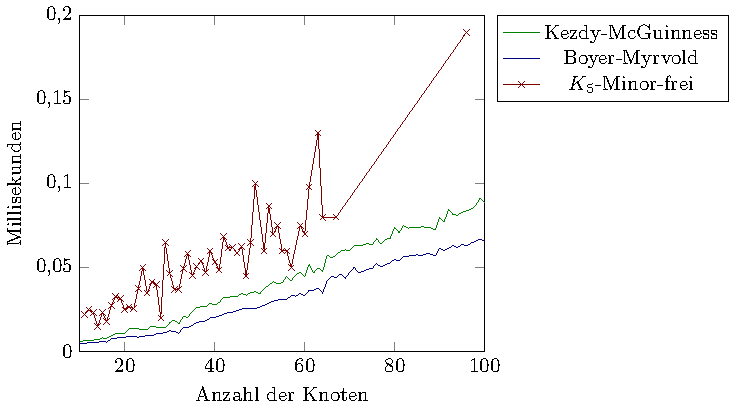
\includegraphics[width=\textwidth,height=\textheight,keepaspectratio]{plots/Benchmarks_Rome.pdf}
  \caption{Benchmark mit den Graphen der Rome Library.}
  \label{fig:Benchmarks-Rome}
\end{figure}

In \Abb \ref{fig:Benchmarks-Rome} ist die Laufzeit in Millisekunden pro Graph zu sehen.
Es fällt auf, dass sich die Laufzeit vom Kezdy-McGuinness-Algorithmus (grün) stark an der des Planaritätstests (blau) orientiert und damit eher linear als quadratisch ist.
Die theoretische Worst-Case-Laufzeit tritt in diesem Anwendungsfall selten auf, da, wie in \Abb \ref{fig:Statistics-Rome} zu sehen, die meisten Graphen entweder planar sind oder einen \kf-Minor enthalten.
Ist ein Graph planar, kann der Algorithmus nach einmaligem Ausführen des Planaritätstests beendet werden, sodass die Laufzeit fast identisch zu der des Planaritätstests ist.
Der Mehraufwand begründet sich in dem Aufbauen der nötigen Datenstrukturen wie der Wagner-Struktur oder einer Kopie des Eingabegraphen, die aus $3$-zusammenhängende Komponenten besteht.
Außerdem findet der Planaritätstest oft direkt einen \kf-Minor oder einen \kdd-Minor, der kein \dd-Separator ist, sodass auch in den beiden Fällen der Kezdy-McGuinness-Algorithmus nach nur einem Rekursionsschritt terminieren kann.
\Abb \ref{fig:Statistics-Rome} ist zu entnehmen, dass viele Graphen entweder einen \kf-Minor enthalten oder planar sind.
Deshalb wurde in \Abb \ref{fig:Benchmarks-Rome} der Kezdy-McGuinness-Algorithmus (rot) zusätzlich nur auf den \kf-Minor-freien Graphen, die nicht planar sind, ausgeführt.
Da nicht für alle Knotenanzahlen solche Graphen vorliegen, wurden gemessenen Werte durch Kreuze markiert.
Hier wird deutlich, dass der Algorithmus deutlich länger läuft, weil der Planaritätstest \dd-Separatoren findet und rekursiv auf die augmentierten Komponenten angewendet wird.
Generell ist in \Abb \ref{fig:Statistics-Rome} aber zu sehen, dass \dd-Separatoren nur in weniger als $10\%$ der Graphen vorkommen.

\begin{figure}[H]
  \centering
  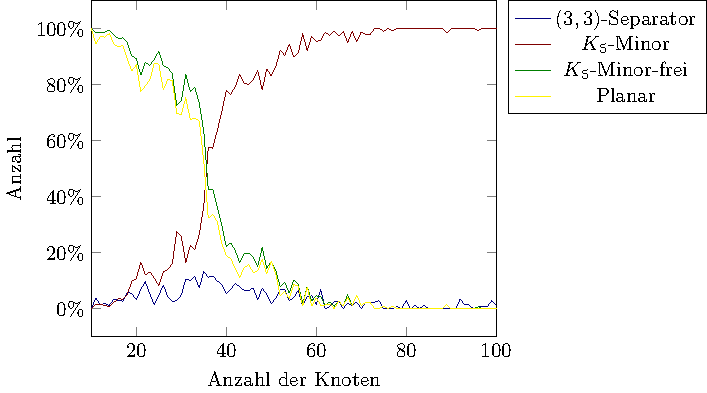
\includegraphics[width=\textwidth,height=\textheight,keepaspectratio]{plots/Statistics_Rome.pdf}
  \caption{Angaben, wie viele Graphen \dd-Separatoren und/oder \kf-Minor enthalten \bzw wie viele planar und/oder \kf-Minor-frei sind.}
  \label{fig:Statistics-Rome}
\end{figure}

\begin{figure}[H]
  \centering
  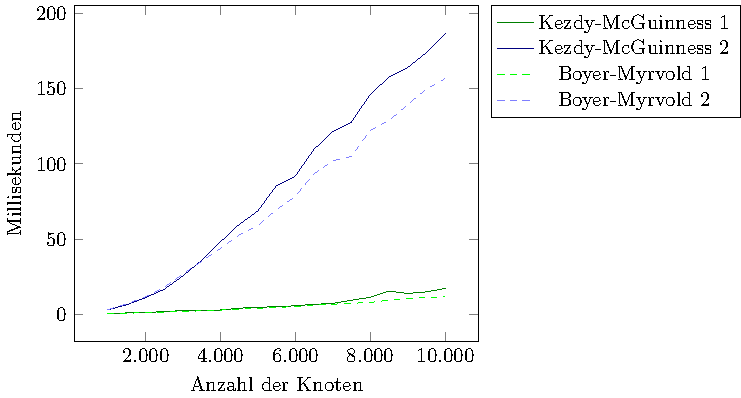
\includegraphics[width=\textwidth,height=\textheight,keepaspectratio]{plots/Benchmarks_Triconnected.pdf}
  \caption{Benchmark $3$-zusammenhängender Graphen mit $n$ Knoten und $2*n$ Kanten (grün) \bzw $10*n$ Kanten.}
  \label{fig:Benchmarks-Triconnected}
\end{figure}

\begin{figure}[H]
  \centering
  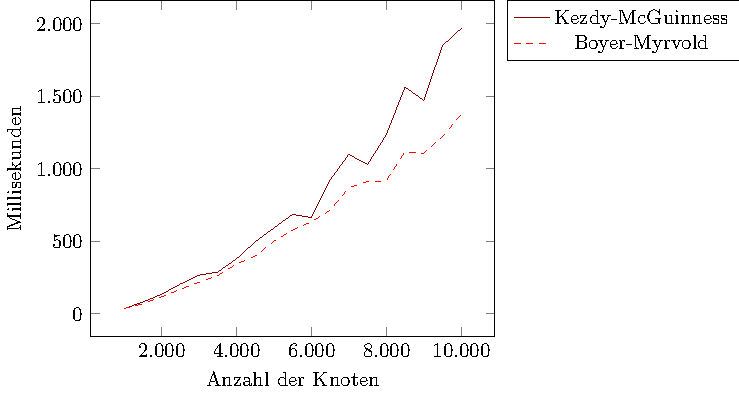
\includegraphics[width=\textwidth,height=\textheight,keepaspectratio]{plots/Benchmarks_TriconnectedVeryDense.pdf}
  \caption{Benchmark $3$-zusammenhängender Graphen mit $n$ Knoten und $f * n$ Kanten für $30 \leq f \leq 100$.}
  \label{fig:Benchmarks-Triconnected-Very-Dense}
\end{figure}

In \Abb \ref{fig:Benchmarks-Triconnected} und \Abb \ref{fig:Benchmarks-Triconnected-Very-Dense} sind die Laufzeiten für größere Graphen zu sehen.
Es wurden für $20$ unterschiedliche Knotengrößen jeweils $25$ Graphen erzeugt und die Messwerte gemittelt.
Die Messungen in \Abb \ref{fig:Benchmarks-Triconnected} decken sich mit den Erkennntnissen, die aus der Rome-Library gewonnen wurden.
Die Graphen in \Abb \ref{fig:Benchmarks-Triconnected-Very-Dense} für größere Kantenanzahlen variieren dagegen deutlicher.
Vermutlich wird für die langsameren Instanzen durch den Planaritätstest ein \kdd-Minor gefunden.
Würde er einen \dd-Separator bilden, müsste die Laufzeit deutlich langsamer sein, wie etwa die Messungen für \kf-Minor-freie Graphen in \Abb \ref{fig:Benchmarks-Rome} zeigen.
Allerdings funktioniert der Test, ob der \kdd-Minor ein \dd-Separator ist, über Tiefensuchen, die durch die deutlich höhere Kantenanzahl länger laufen.
Es sei außerdem erwähnt, dass durch die hohe Kantenanzahl immer ein \kf-Minor enthalten ist.

\ \\

Zuletzt wurden in \Abb \ref{fig:Benchmarks-Small} Graphen mit wenigen Knoten und Kanten getestet.
Es wurden nur $10$ Graphen pro Knotenanzahl erzeugt, dafür jedoch in einem kleineren Intervall.
Dadurch konnte eine stärkere Varianz in der Laufzeit gemessen werden.
In \Abb \ref{fig:Statistics-Small} wurde angegeben, wie viele \dd-Separatoren durchschnittlich gefunden wurden.
Es zeichnet sich ab, dass der Kezdy-McGuinness-Algorithmus schneller ist, umso weniger \dd-Separatoren gefunden werden.
Beispielsweise enthielten von den Graphen mit $700$ Knoten im Schnitt $30\%$ einen \dd-Separator, die Laufzeit lag bei $0,685ms$.
Demgegenüber enthielt keiner der Graphen mit $720$, bis $740$ Knoten einen \dd-Separator, sodass eine schnellere Laufzeit abgelesen werden kann.
Die Laufzeit für Graphen mit $740$ Knoten lag beispielsweise bei nur $0,532ms$ und liefen damit ähnlich schnell, wie die für kleineren Instanzen mit $580$ Knoten.

\begin{figure}[H]
  \centering
  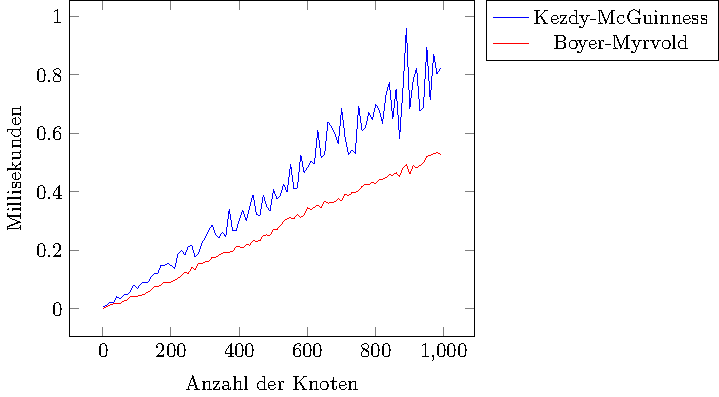
\includegraphics[width=\textwidth,height=\textheight,keepaspectratio]{plots/Benchmarks_Small.pdf}
  \caption{Benchmark für Graphen mit $n$ Knoten und $2*n$ Kanten.}
  \label{fig:Benchmarks-Small}
\end{figure}

\begin{figure}[H]
  \centering
  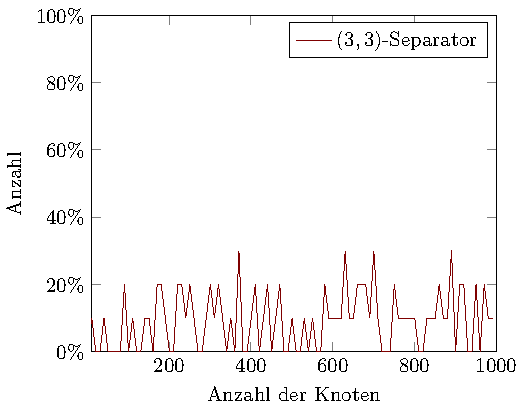
\includegraphics[width=\textwidth,height=\textheight,keepaspectratio]{plots/Statistics_Small.pdf}
  \caption{Angabe, wie viele Graphen mit $n$ Knoten und $2*n$ Kanten einen \dd-Separatoren enthalten.}
  \label{fig:Statistics-Small}
\end{figure}

% fazit.tex
\chapter{Zusammenfassung und Ausblick}
\label{cha:fazit}

Es wurde ein Verfahren vorgestellt, das entscheiden kann, ob ein Graph einen \kf-Minor enthält.
Außerdem wurde erklärt, wie sich \kf-Minor-freie Graphen nach dem Theorem von Wagner aufteilen lassen und eine Baumstruktur gezeigt, die diese Aufteilung widerspiegelt.
Für die Implementierung in OGDF wurden im Wesentlichen Block-Cut Trees und SPQR-Bäume verwendet, um $3$-zusammenhängende Graphen zu erzeugen, und anschließend der Boyer-Myrvold Planaritätstest, um solange \dd-Separatoren zu finden, bis ein \kf-Minor gefunden wurde oder der Graph eindeutig \kf-Minor-frei ist.
Bisher werden Zertifikate für $3$-zusammenhängende Graphen, die \kf-Minor-frei sind, erzeugt.
Vor allem die Berechnung von \kf-Modellen im Eingabegraph kann im Hinblick auf den praktischen Nutzen von wesentlicher Bedeutung sein.
Auch kann es für einige praktische Anwendungen sinnvoll sein, den Algorithmus zu erweitern, sodass mehrere \kf-Minoren in Graphen zu berechnen werden können.
Dafür könnte der Algorithmus \zB so angepasst werden, dass in gefundenen \kf-Minoren einzelne Kanten verändert (kontrahiert, entfernt) werden, um bei einem erneuten Durchlauf einen anderen \kf-Minor zu finden.
So könnten viele \kf-Minoren gefunden werden, die sich allerdings kaum unterscheiden und eine hohe Laufzeit verursachen.
Ein weiterer Ansatz könnte daraus bestehen, den Algorithmus nicht zu terminieren, wenn in einer augmentierten Komponente ein \kf-Minor gefunde wurde.
Wird stattdessen in den übrigen Komponenten weitergesucht, ist es möglich, \kf-Minoren zu finden, die sich stark voneinander unterscheiden.
Tests während der experimentellen Analyse haben jedoch angedeutet, dass auf diese Art meist nur einstellige Mengen von \kf-Minoren in den getesteten Graphen gefunden werden konnten.
Da es sich um ein heuristisches Verfahren handelt, wurde es nicht mit in die Arbeit aufgenommen -- einige praktische Anwendungen, wie die Berechnung des maximalen Schnittes in Graphen, die nicht \kf-Minor-frei sind, könnten jedoch davon profitieren.
Es steht aus, diese beiden Ansätze in einer experimentellen Analyse für solche speziellen Anwendungsfälle zu prüfen.

Darüber hinaus gibt es Ansätze in \cite{Li11}, \cite{ReL08} und \cite{ReL}, die in theoretisch linearer Laufzeit entscheiden, ob ein Graph \kf-Minor-frei ist.
Allerdings bleibt die Frage offen, ob eine Implementierung in der Praxis eine bessere Laufzeit aufweisen würde, da teils mit großen Konstanten gearbeitet wird.

Letztlich wären weitere Laufzeittests speziell für Graphen, die nicht planar sind und keinen \kf-Minor enthalten, interessant, da vor allem dann hohe Laufzeiten in der Praxis auftreten können.
Für alle getesteten Graphen konnte der Algorithmus dagegen in wenigen Sekunden entscheiden, ob ein \kf-Minor in einem Graph enthalten ist.


% Anhang (optional)
\appendix
% anhang.tex
\chapter{Weitere Informationen}


%Abbildungsverzeichnis
\listoffigures
\addcontentsline{toc}{chapter}{Abbildungsverzeichnis}
\cleardoublepage

% Algorithmenverzeichnis
\listofalgorithms
\addcontentsline{toc}{chapter}{Algorithmenverzeichnis}
\cleardoublepage

% Symbolverzeichnis (optional)
\renewcommand{\symheadingname}{Symbolverzeichnis}
\listofsymbols
\addcontentsline{toc}{chapter}{Symbolverzeichnis}
\cleardoublepage

% Literaturverzeichnis
\bibliographystyle{gerplain}
\bibliography{options/literatur}
\addcontentsline{toc}{chapter}{\bibname}

% Erklaerung
\thispagestyle{myheadings}
%\markboth{}{ERKLÄRUNG}
%\addcontentsline{toc}{chapter}{Erklärung}
\markboth{}{EIDESSTATTLICHE VERSICHERUNG}
\addcontentsline{toc}{chapter}{Eidesstattliche Versicherung}
% erklaerung.tex
\parindent 0pt
\cleardoublepage

{\centering \hspace*{1cm}\Large \textbf{Eidesstattliche Versicherung} 

}

\normalsize
\vspace*{1cm}

\parbox{5cm}{ \centering \MeinNachname, \MeinVorame 
\vspace*{0,1cm}
\hrule
\vspace*{0,1cm}
\strut \small \ Name, Vorname} \hfill
\parbox{3cm}{ \centering \MeineMatrikelnummer 
\vspace*{0,15cm}
\hrule
\vspace*{0,1cm}
\strut \small \ Matr.-nr.}

\vspace*{1cm}

Ich versichere hiermit an Eides statt, dass ich die vorliegende \MeineArbeit mit dem Titel

\vspace{0,25cm}
{
\centering
\textbf{\MeinTitel}

}
\vspace{0,25cm}

selbstständig und ohne unzulässige fremde Hilfe erbracht habe. Ich habe keine anderen als die angegebenen Quellen und Hilfsmittel benutzt sowie wörtliche und sinngemäße Zitate kenntlich gemacht. Die Arbeit hat in gleicher oder ähnlicher Form noch keiner Prüfungsbehörde vorgelegen. 
\vspace*{1cm}

\parbox{6.2cm}{ Dortmund, den \today
\vspace*{0,1cm}
\hrule
\vspace*{0,2cm}
\strut \small \ Ort, Datum} \hfill
\parbox{5cm}{ \color{white} Platzhalter \color{black}
\vspace*{0,1cm}
\hrule
\vspace*{0,2cm}
\strut \small \ Unterschrift}

\vspace*{1,5cm}

\textbf{Belehrung:} \vspace{0,25cm}
\newline
Wer vorsätzlich gegen eine die Täuschung über Prüfungsleistungen betreffende Re\-ge\-lung einer Hochschulprüfungsordnung verstößt, handelt ordnungswidrig. Die Ordnungs\-widrig\-keit kann mit einer Geldbuße von bis zu 50.000,00 \euro\ geahndet werden. Zuständige Verwaltungsbehörde für die Verfolgung und Ahndung von Ordnungswidrigkeiten ist der Kanzler/ die Kanzlerin der Technischen Universität Dortmund. Im Falle eines mehrfachen oder sonstigen schwerwiegenden Täuschungsversuches kann der Prüfling zudem exmatrikuliert werden. (\textsection\ 63 Abs. 5 Hochschulgesetz - HG - )
\vspace{0,25cm} \newline
Die Abgabe einer falschen Versicherung an Eides statt wird mit Freiheitsstrafe bis zu 3 Jahren oder mit Geldstrafe bestraft.
\vspace{0,25cm} \newline
Die Technische Universität Dortmund wird gfls. elektronische Vergleichswerkzeuge (wie z.B. die Software „turnitin“) zur Überprüfung von Ordnungswidrigkeiten in Prüfungsverfahren nutzen.
\vspace{0,25cm} \newline
Die oben stehende Belehrung habe ich zur Kenntnis genommen:
\vspace*{1cm}

\parbox{6.2cm}{ Dortmund, den \today
\vspace*{0,1cm}
\hrule
\vspace*{0,1cm}
\strut \small \ Ort, Datum} \hfill
\parbox{5cm}{ \color{white} Platzhalter \color{black}
\vspace*{0,1cm}
\hrule
\vspace*{0,1cm}
\strut \small \ Unterschrift}

%
%\addcontentsline{toc}{chapter}{Eidesstattliche Versicherung}


%\cleardoublepage
%\textbf{
%Die unten stehende Erklärung ist nur für Diplomarbeiten geeignet.
%Für Bachelor- und Masterarbeiten diese Seite vollständig aus der Arbeit entfernen und stattdessen die vorgebene Erklärung vom Prüfungsamt mit in die Arbeit einbinden.
%Diese muss nicht im Inhaltsverzeichnis auftauchen und muss auch keine Seitenzahl haben.
%Einfach nur das ausgefüllte Blatt ganz am Ende mit in die Arbeit einbinden.
%Die Erklärung findet sich auf der Seite des Prüfungsamts (TU Homepage $\rightarrow$ Studierende $\rightarrow$ Prüfungsangelegenheiten) unter dem Punkt Bachelor- und Masterarbeiten.
%Diesen fett gedruckten Text auf jeden Fall aus der Arbeit entfernen!
%}
%\\
%\normalsize
%Hiermit versichere ich, dass ich die vorliegende Arbeit selbstständig verfasst habe und keine anderen als die angegebenen Quellen und Hilfsmittel verwendet sowie Zitate kenntlich gemacht habe.\\\\
%Dortmund, den \today \\\\\\\\
%Muster Mustermann
% EOF
\cleardoublepage

\end{document}
% EOF
